\chapter{EvoOracle: LLMs for Oracles}
\label{cha:evoOracles}
\vspace{0.4 cm}

In this chapter, we introduce EvoOracle, our approach designed for potential oracle generation using Large Language Models and outline its design. To initiate the process, it requires some preprocessing, including analyzing projects, parsing source code, and extracting the necessary information for use in the generation process. The focal method needs to pass through the tool's components to generate a correct Oracle. The components of EvoOracle and the process overview will be described in the following sections.

\section{Components of EvoOracle}
\label{sec:components}
\vspace{0.2 cm}
EvoOracle is designed with a some components what work together to to generate test cases and test Oracles for a given projects. Figure~\ref{fig:evooracle_overview} provides an overview of EvoOracle's key components. Each of the components are explained in details below:

\begin{enumerate}
    \item \textbf{SUT Processor:} This component takes the SUT and performs analysis on the code by parsing it. Also, it prepares a dataset of all the metadata of the project by mapping all the classes, methods, arguments, code comments etc all the relevant information. Later, it also removes assertions from the test cases and substitutes them with placeholders. 
    
    \item \textbf{Automated Test Generator:} This component generates the test suite for each target class based on the specified criterion like line coverage, branch coverage etc, configuration and budget.
    
    \item \textbf{Prompt Processor:} Prompt Processor component takes these test cases, now equipped with placeholders and focal methods, and formulates context for LLM prompting.
    
    \item \textbf{LLM Query Processor:} The LLM Query Processor component utilizes this context to prompt the LLMs using the LLM interface, later, passing the generated responses to the LLM Response Handler component.
    
    \item \textbf{LLM Interface:} The LLM interface provides supports for services from the LLMs. This interface can be connected with models or APIs.
    
    \item \textbf{LLM Response Handler:}
    
    \item \textbf{Test Executor:} Test Executor compiles and executes the test cases.
    
    \item \textbf{Evaluator:} This component follows heuristics to evaluate the quality of the generated tests. Firstly, it checks if the generated test case is syntactically correct. Secondly, it check if the test compiles. Finally, it checks if the test runs without any errors. This is already an indication that the candidate tests are good enough. Another criteria is to run mutation testing on the generated tests.
\end{enumerate}

\begin{figure}[H]
\centering
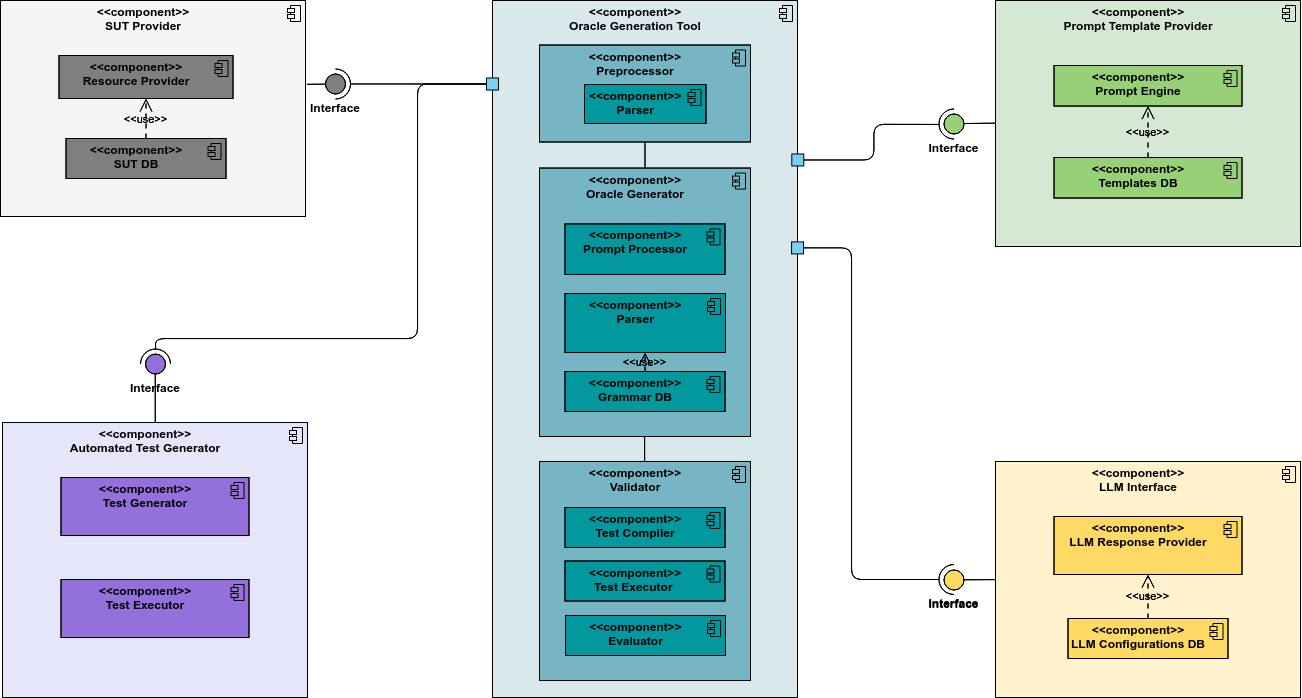
\includegraphics[width=1\textwidth]{images/EvoOracle_ components.png}
\caption{Components of our proposed tool: EvoOracle}
\label{fig:component_diagram}
\end{figure}

\section{Workflow}
\label{sec:workflow}
\vspace{0.2 cm}

To initiate the process, we acquire a dataset of Java projects sourced from GitHub. Employing automated test case generation tools such as EvoSuite and Randoop, we systematically create Automated JUnit Test Cases for each project, laying the foundation for EvoOracle's subsequent operations. The tool begins by extracting metadata linked to the identified classes and methods within each project. Subsequently, it mines test cases and establishes mappings with corresponding focal methods extracted from the earlier project analysis. The SUT (System Under Test) Processor component plays a pivotal role in this phase, removing assertions from the test cases and substituting them with placeholders. Following this, the Prompt Processor component takes these test cases, now equipped with placeholders and focal methods, and formulates context for LLM prompting. The LLM Query Processor component utilizes this context to prompt the LLMs, passing the generated responses to the LLM Response Handler component. This handler, in turn, readies the test cases for execution. Finally, the Test Executor compiles and executes the newly generated tests, completing the comprehensive cycle of EvoOracle's oracle generation process.

designed an adaptive focal context generation mechanism, which generates a context containing as much as necessary information for the focal method, while leaving enough space for ChatGPT to produce complete responses. To tackle the second limitation, we implemented a validation component and a repair component. The validation component includes a parser, compiler, and test executor. The repair component consists of rule-based repair and ChatGPT-based repair. Rule-based repair addresses simple errors such as syntax errors and missing import statements. If rule-based repair fails, ChatUniTest resorts to ChatGPT-based repair. It constructs a prompt with an error message, incorrect unit test, and adaptive focal context to obtain the corrected unit test from ChatGPT. If a test remains unfixed after several validation and repair rounds, it is marked as deprecated.

\begin{figure}[H]
    \centering
    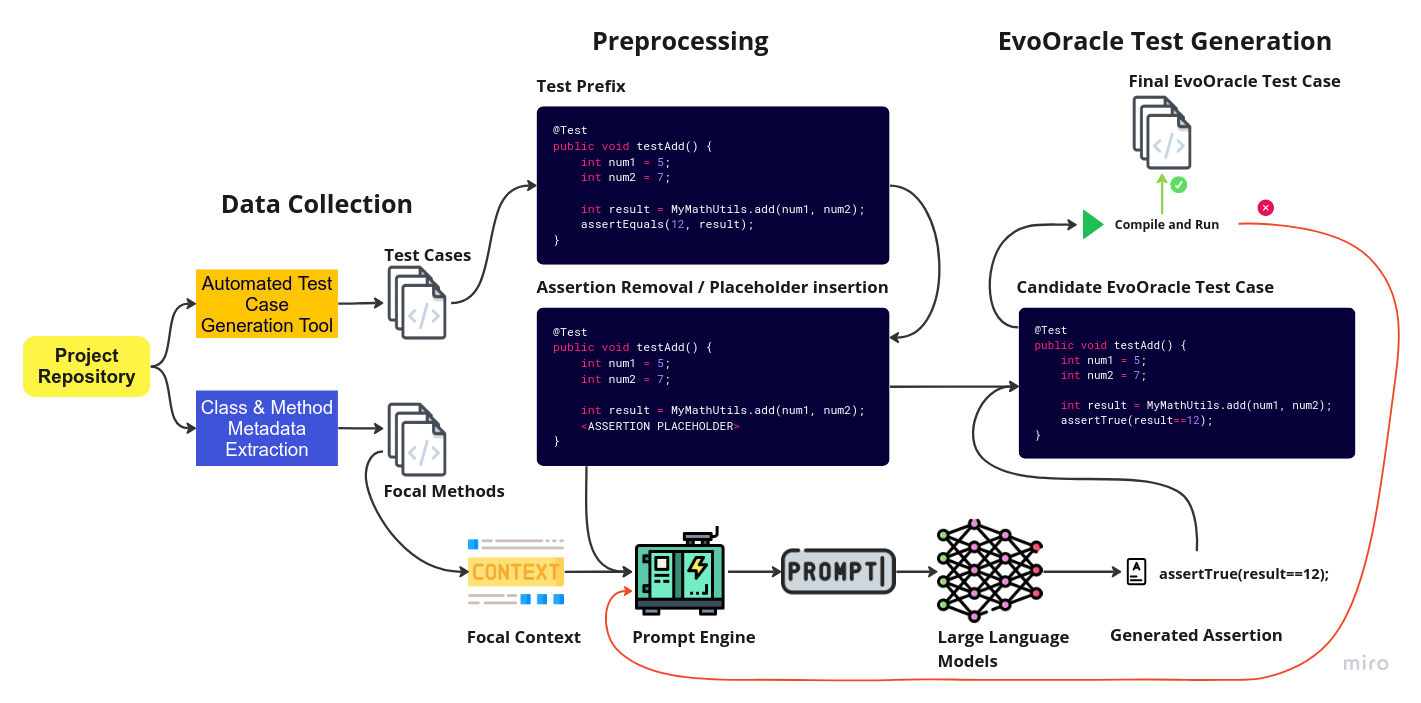
\includegraphics[width=1\linewidth]{images/evooracle_overview.png}
    \caption{Overview of EvoOracle}
    \label{fig:evooracle_overview}
\end{figure}



In the following sub-chapters, we will delve into the intricacies of each step, providing detailed descriptions and insights into the nuances of EvoOracle's comprehensive process.

